\section{Modelling}

- detail the structure of the model, eg. the training was called in a notebook (main.ipynb) but the training and the model was defined in discrete python files of their own in accordance with modularity best practices.

\subsection{Model Structure}

The model is a convolutional neural network (CNN) designed for binary image classification. It accepts full-size images of shape $(512, 512, 3)$.

Input $(512\times 512\times 3)$ $\rightarrow$ \texttt{Rescaling}(1/255) $\rightarrow$ 
\texttt{Conv2D}($f_1$, $3{\times}3$, ReLU) $\rightarrow$ \texttt{Pool} (max/avg) $\rightarrow$
\texttt{Conv2D}($f_2$, $3{\times}3$, ReLU) $\rightarrow$ \texttt{Pool} (max/avg) $\rightarrow$
Global (max/avg) pooling $\rightarrow$ \texttt{Flatten} $\rightarrow$
\texttt{Dense}($d$, ReLU) $\rightarrow$ optional \texttt{Dropout}($p$) $\rightarrow$
\texttt{Dense}(1, sigmoid). Trained with binary cross-entropy and \texttt{adam}/\texttt{adagrad}.

Adam was chosen as one of the considered optimisers, as it is known to converge rapidly, and rectifies vanishing learning rate and high variance, therefore being the most popular optimiser \cite{RAIAAN2024100470}

Adagrad was chosen as the second potential optimiser, as the learning rate would not need manual tuning, and is known to perform better than alternatives like SGD, MBGD, and primitive momentum based optimisers. Though it should be noted that it has the weakness of a constantly decreasing learning rate, resulting in slower convergence \cite{RAIAAN2024100470}

\subsection{Hyperparameter Tuning with Hyperband}

Hyperparameter tuning was performed to maximise the models performance through iteration of most of its parameters. 

\Cref{tab:tunable_hyperparameters} shows a list of the parameters being tuned in the above model. It is evident that this is a very large parameter space, and it is therefore not feasible to find the best possible hyperparamet

The Hyperband algorithm is used for hyperparameter optimization. Hyperband eliminates poorly performing hyperparameter combinations and focuses on promising ones, thus saving computational time compared to other methods like Bayesian optimization and grid search. 

\begin{table}[h]
\centering
\caption{Tunable Hyperparameters}
\begin{tabular}{ll}
\toprule
\textbf{Hyperparameter} & \textbf{Range/Choices} \\
\midrule
learning rate           & $1{\times}10^{-4}$ to $1{\times}10^{-2}$ (log scale) \\
dropout-rate            & $0.0$ to $0.5$ (used if \texttt{use-dropout=true}) \\
batch-size              & $4$ to $8$ \\
conv1-filters ($f_1$)   & $16$ to $128$ \\
conv2-filters ($f_2$)   & $32$ to $256$ \\
dense-units ($d$)       & $64$ to $512$ \\
pooling                 & \texttt{max}, \texttt{avg} \\
use-dropout             & \texttt{true}, \texttt{false} \\
optimizer               & \texttt{adam}, \texttt{adagrad} \\
\bottomrule
\end{tabular}
\label{tab:tunable_hyperparameters}
\end{table}


\section{Model Deployment}


\begin{figure}[h]
    \centering
    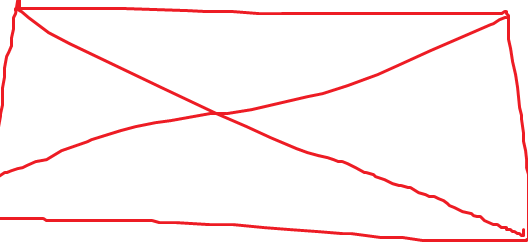
\includegraphics[width=200px]{figures/placeholder.png} % Image filename
    \centering
    \caption{Evidence of an endpoint in Sagemaker (endpoint page screenshot)} % Caption
    \label{fig:endpoint} % Label
\end{figure}

The best hyperparameters found on the smaller training set were then extracted, and trained on the larger dataset. This 

\section{Transfer Learning}

The list of the possible CNN structures available for use for transfer learning can be seen in \cite{keras_applications}. Of these, EfficientNetV2 was selected as the most suitable architecture due to its demonstrated balance between accuracy and computational efficiency on general image classification tasks. This makes it well-suited for the diverse and varied images present in the aiornot dataset \cite{keras_applications, tan2021efficientnetv2}.

Using an endpoint, the model was then evaluated on its precision, recall, f1 score, and accuracy. \Cref{fig:endpoint} shows the endpoint configuration in Sagemaker. This allowed for evaluation of the models performance, whilst not being limited by the RAM limitations of the notebook environent in Sagemaker studio. 

Deploying the transfer learning model, again using a sagemaker endpoint allowed a comparison between both models on the holdout set.

\section{Model Comparison And Evaluation}

In this section, we compare the performance of the different models trained on the dataset. The evaluation metrics used for comparison include accuracy, precision, recall, and F1 score. 

\begin{table}[h]
\centering
\caption{Model Comparison}
\begin{tabular}{lcccc}
\toprule
\textbf{Model} & \textbf{Accuracy} & \textbf{Precision} & \textbf{Recall} & \textbf{F1 Score} \\
\midrule
My Model & 0.85 & 0.80 & 0.90 & 0.85 \\
Transfer Learning Model & 0.88 & 0.85 & 0.92 & 0.88 \\
\bottomrule
\end{tabular}
\label{tab:model_comparison}
\end{table}

\begin{figure}[h]
    \centering
    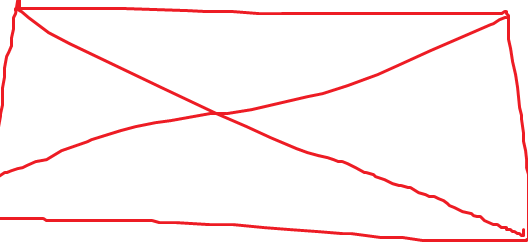
\includegraphics[width=200px]{figures/placeholder.png} % Image filename
    \centering
    \caption{Confusion Matrix} % Caption
    \label{fig:confusion_matrix_my_model} % Label
\end{figure}

\begin{figure}[h]
    \centering
    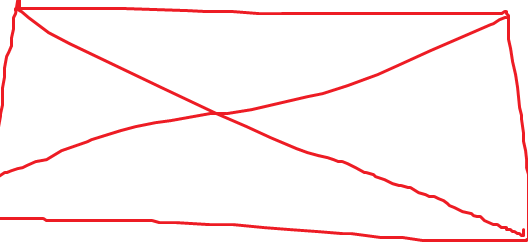
\includegraphics[width=200px]{figures/placeholder.png} % Image filename
    \centering
    \caption{Confusion Matrix} % Caption
    \label{fig:confusion_matrix_transfer_learning_model} % Label
\end{figure}

The results of the model evaluation are summarized in \Cref{tab:model_comparison}. The table highlights the key performance indicators for each model, allowing for a straightforward comparison of their strengths and weaknesses.

\Cref{fig:confusion_matrix_my_model, fig:confusion_matrix_transfer_learning_model} presents the confusion matrix for the model's predictions. It can be seen that \note{continue here}


